\documentclass[11pt,twoside,a4paper]{article}
\usepackage[utf8]{inputenc}
%\usepackage[english,german]{babel}
%\usepackage{utopia}
\usepackage[margin=1in]{geometry}
\usepackage[parfill]{parskip}
\usepackage{makeidx}
\usepackage[onehalfspacing]{setspace}
\usepackage{fancyhdr}
\usepackage{lastpage}
\usepackage{hyperref}
\usepackage{graphicx}
\usepackage[sf,bf]{titlesec}
\renewcommand{\rmdefault}{ptm}
\renewcommand{\sfdefault}{phv}
\renewcommand{\familydefault}{\rmdefault}
\newcommand{\titleText}{Film DNS}
\newcommand{\authorText}{Patrick Guenthard}
\newcommand{\dateText}{\today}



\title{\titleText}
\author{\authorText}
\date{\dateText}

\pagestyle{fancy}
\fancyhf{}

\fancyhead[EL]{\titleText}
\fancyhead[OR]{\authorText}
\cfoot{\thepage \space von \pageref{LastPage}}

\begin{document}
\maketitle
\tableofcontents

\section{Aufgabestellung}

\section{Theorie}

\subsection{Geschichte}

\textit{DNS} ist zur Zeit des \textit{ARPANETs}\footnote{\cite{arpanetwiki}} entstanden. ARPANET basierte wie das heutige Internet auf dem IP Protokoll. In diesem schnell wachsenden Netzwerk [Figure: \ref{arpanet77}] wurden Methoden gesucht, um die vielen IP-Addressen zu verwalten. Das \textbf{Stanford Research Institute} hatte  das \texttt{hosts}-File\footnote{Unix: \texttt{/etc/hosts} Windows: \texttt{C:\textbackslash Windows\textbackslash System32\textbackslashdrivers\textbackslash etc\textbackslash host}} eingeführt welches die IPs auf selbst definierte Host-Names mappte\footnote{\cite{dnswiki} Abs. \textit{History}}. Diese Lösung war hatte mehrere Probleme: Sie war umständlich, und dezentral da jede Maschine ein eigenes \texttt{hosts} File besass. 

\begin{figure}
  \center
  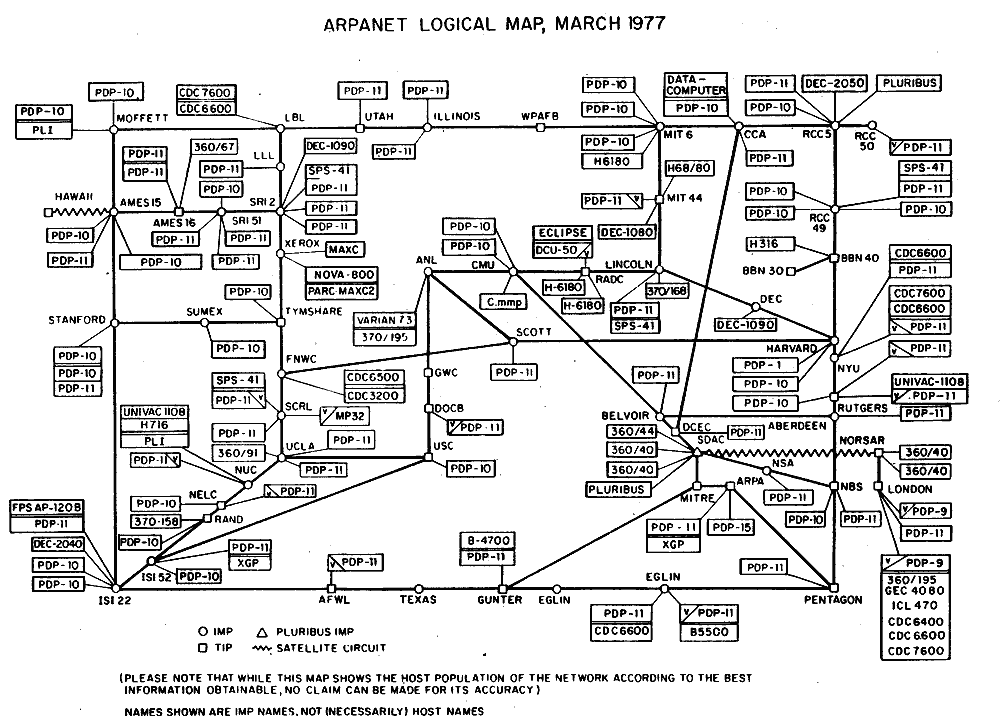
\includegraphics[width=8cm]{arpanet77}
  \caption{ARPANET, März 1977 \label{arpanet77}}
\end{figure}

Es wurde nach einer zentralen und vor allem automatisierten Lösung gesucht. 1983 wurde an der \textit{UC Irvine} mit der Entwicklung von DNS begonnen. Im selben Jahr wurde auch eine erste Implementierung geschrieben.

1984 wurde an der UC Berkeley eine UNIX Implementierung geschrieben. Die \textit{Berkeley Internate Name Domain (BIND)} Server Software verbreitete sich sehr schnell und ist noch heute einer der meist verbreiteten DNS Server Weltweit. 

\subsection{Funktionalität}



\section{Vorgehen Installation}


\section{Ergebnis}

\section{Testprotokoll}


\section{Reflexion}



\begin{thebibliography}{9}

\bibitem[DNSWIKI]{dnswiki} \href{https://en.wikipedia.org/wiki/Domain_Name_System}{\textbf{Domain Name System} auf \textbf{Wikipedia}}, zuletzt abgerufen: 26.5.2016

\bibitem[ARPANETWIKI]{arpanetwiki} \href{https://en.wikipedia.org/wiki/Domain_Name_System}{\textbf{ARPANET} auf \textbf{Wikipedia}}, zuletzt abgerufen: 26.5.2016
    
\end{thebibliography}



\end{document}